\documentclass[11pt,class=report,crop=false]{standalone}
\usepackage[screen]{../logic}

\begin{document}

%====================================================================
\chapitre{Codage de Gödel} 
%====================================================================

\objectifs{On transforme les symboles, les formules et même les preuves en des entiers. On expliquera ensuite les grandes lignes de la preuve du premier théorème d'incomplétude.} 


\index{codage de Godel@codage de Gödel}

%%%%%%%%%%%%%%%%%%%%%%%%%%%%%%%%%%%%%%%%%%%%%%%%%%%%%%%%%%%%%%%%%%
\section{Codage des symboles, formules, preuves}

%--------------------------------------------------------------------
\subsection{Motivation} 

Le but est de coder chaque formule par un entier, afin de permettre un traitement mathématique et algorithmique. 
Une analogie parlante se fait avec le code ASCII qui code un caractère par un entier (`A': 65, `B' : 66, \dots). 
Pour coder un texte (une chaine de caractères), il suffit de juxtaposer les entiers (`BAC' : 66/65/67). 
Comme un ordinateur ne code pas les entiers par les chiffres de 0 à 9 mais seulement avec les symboles 0 et 1, nos caractères ASCII sont écrits sur 8 bits :
\begin{center}
\begin{tabular}{cc}
A :& 01000001 \\
B :& 01000010 \\
Z :& 01011010
\end{tabular}
\end{center} 

Pour une chaine de caractères il suffit de juxtaposer les codes de chaque caractère en un seul entier. 
\mycenterline{
`BAC' \quad : \quad  010000100100000101000011 
}
Le décodage est facile et commence par séparer le code par paquets de 8 bits. 

\medskip

Il y a une distinction importante à faire entre un nombre et la représentation de ce nombre : 
\mycenterline{
7, \quad VII, \quad sept, \quad $111_2$, \quad SSSSSSS(0)
 }
 sont différentes représentations du même entier désigné par `7' (ici en chiffres arabes, romains, en toutes lettres, en écriture binaire et dans le langage $\mathcal{L}_0$ de l'arithmétique de Peano). C'est une distinction bien connue en informatique.
 Il y a un aspect philosophique profond à donner un nom aux choses, même si le nom ne change pas la chose elle-même. Ainsi, tout comme le mot \emph{table} n'a pas quatre pieds, les symboles arithmétiques servent uniquement de support formel pour représenter les entiers. 

Dans la suite, ce qui est vraiment fondamental c'est l'existence d'un codage et d'un décodage. 
Les rouages internes ne sont pas si importants et varient d'un livre à l'autre.  
De toute façon, on verra que ce codage est absolument inutilisable en pratique. 

%--------------------------------------------------------------------
\subsection{Coder les symboles} 

On considère le langage $\mathcal{L}_0 = (0,S,+,\times)$ de la logique du premier ordre pour l'arithmétique de Peano. 
Il faut coder les symboles du langage, les connecteurs, les quantificateurs et les variables $(x_i)_{i\ge1}$. 

On choisit (arbitrairement) le codage suivant (voir le livre de Peter Smith) : 

\begin{center}
\begin{tabular}{cccccccccccccc}
$\lnot$ & $\land$ & $\lor$ & $\limplies$ & $\lequiv$ & $\forall$ & $\exists$ & $=$ & $($ & $)$ & $0$ & $S$ & $+$ & $\times$ \\ 
1 & 3 & 5 & 7 & 9 & 11 & 13 & 15 & 17 & 19 & 21 & 23 & 25 & 27
\end{tabular}
\end{center} 

\begin{center}
\begin{tabular}{cccccc}
$x_1 / x$ & $x_2 / y$ & $x_3 / z$ & $x_4$ & $\cdots$ & $x_i$\\ 
$2$ & $4$ & $6$ & $8$ & $\cdots$ & $2i$ 
\end{tabular}
\end{center} 

Par exemple, le code du symbole \og{}$\exists$\fg{} est $c=13$. 
Le symbole du code $c=21$ est \og{}0\fg{} (la constante zéro du langage). 
La variable $x_i$ est codée par l'entier $2i$. 

Pour décoder un code, il suffit de lire le tableau de bas en haut : 
\begin{itemize}
    \item si $c$ est impair, chercher à quel symbole il correspond, 
    \item si $c$ est pair, le symbole est la variable $x_{c/2}$. 
\end{itemize}

Remarques :
\begin{itemize}
    \item Pour certaines preuves on peut limiter le nombre de connecteurs, par exemple à $(\lnot, \limplies, \forall)$ ou bien à $(\lnot, \lor, \forall)$. 
    \item Il est important pour le décodage de ne pas avoir de code qui vaut $0$. 
\end{itemize}

%--------------------------------------------------------------------
\subsection{Coder une formule} 

On considère un mot du langage $\mathcal{L}_0$, c'est donc une suite finie de symboles. 
Cela peut être une formule \og{}$\forall S(x)=y$\fg{} ou une suite de symboles qui n'a pas de sens \og{}$S(\forall) \limplies \lnot \times 0$\fg{}. 

On va noter $c_1, c_2, c_3, \ldots$ les codes des symboles de ce mot (lu de gauche à droite). 
Ces codes seront les exposants dans un produit de nombres premiers : 
\[ 2^{c_1} \times 3^{c_2} \times 5^{c_3} \times \cdots \] 

On note $\pi_1=2$, $\pi_2=3$, $\pi_3=5, \ldots$ la suite ordonnée des nombres premiers. 
On peut ainsi formaliser notre construction : 
\begin{itemize}
    \item On part d'un mot (ou d'une formule) $\mathcal{P}$ qui est une suite de symboles $a_1, a_2, \ldots, a_l$ de $\mathcal{L}_0$. 
    \item À chaque symbole $a_i$, on associe son code $c_i$. 
    \item Le \defi{nombre de Gödel}\index{nombre de Godel@nombre de Gödel} $n(\mathcal{P})$ de la formule $\mathcal{P}$ est :
    \mybox{
        $\displaystyle n = \prod_{i=1}^l \pi_i^{c_i}$
    } 
\end{itemize}

Remarques.  
C'est généralement un très grand nombre. 
Cela s'applique aussi à un mot quelconque de $\mathcal{L}_0$, même si ce n'est pas une formule. 


\begin{exemple}
\sauteligne
\begin{itemize}
    \item $\mathcal{P}$ : \og{}$\lnot(x=0)$\fg{} 
    \begin{itemize}
        \item $[a_1, \ldots, a_6] = [\lnot, (, x, =, 0, )]$ 
        \item $[c_1, \ldots, c_6] = [1, 17, 2, 15, 21, 19]$ 
        \item $n(\mathcal{P}) = 2^1 \cdot 3^{17} \cdot 5^2 \cdot 7^{15} \cdot 11^{21} \cdot 13^{19}$ 
    \end{itemize}
    
    \item \og{}2\fg{} n'existe pas dans $\mathcal{L}_0$, son écriture dans $\mathcal{L}_0$ est \og{}$SS0$\fg{} dont le nombre de Gödel est $2^{23} \cdot 3^{23} \cdot 5^{21}$. 
\end{itemize}
\end{exemple}

%--------------------------------------------------------------------
\subsection{Décoder} 

Le décodage est basé sur la décomposition en facteurs premiers des entiers (aussi appelé le principe fondamental de l'arithmétique) et en particulier sur l'unicité de cette décomposition. 

\begin{theoreme}
Pour tout entier $n \ge 1$, il existe un entier $l \ge 1$ et des entiers $\alpha_1, \dots, \alpha_l \ge 0$ tels que : 
\[ n = \pi_1^{\alpha_1} \times \pi_2^{\alpha_2} \times \dots \times \pi_l^{\alpha_l} \] 
De plus, les $\alpha_i$ sont uniques. 
\end{theoreme}

Ainsi, pour décoder un nombre de Gödel $n$, c'est-à-dire retrouver la formule encodée, on commence par décomposer $n$ en produit de facteurs premiers. 
Les exposants $c_1, \dots, c_l$ sont les codes qui redonnent un à un les symboles de la formule. 

Il n'y a qu'une seule façon de décoder un nombre. 
D'un point de vue mathématique, cela signifie que le codage est injectif : 
\[ \text{Si } \ n(\mathcal{P}) = n(\mathcal{Q}) \ \text{ alors } \ \mathcal{P} = \mathcal{Q}. \] 

\begin{exemple}
    $n = 35\,872\,267\,500$ 
    \begin{itemize}
        \item Décomposition en facteurs premiers : $n = 2^2 \times 3^{15} \times 5^4$.
        \item Les exposants donnent les codes $[2, 15, 4]$. 
        \item Chaque code se décode en un symbole $[x, =, y]$. 
        \item La formule de $n$ est donc \og{}$x=y$\fg{}. 
    \end{itemize}
\end{exemple}
    

%--------------------------------------------------------------------
\subsection{Coder les preuves} 

On souhaite aussi coder une preuve entière par un seul entier. 
Une preuve est ici une suite finie de formules $(\mathcal{P}_1, \mathcal{P}_2, \ldots, \mathcal{P}_L)$. 
Comment coder une preuve ? 
Chaque $\mathcal{P}_j$ est codée par son nombre de Gödel $n_j = n(\mathcal{P}_j)$ 
Ensuite, on associe à la preuve son \defi{super-nombre de Gödel}\index{nombre de Godel@nombre de Gödel} : 
\[ N = 2^{n_1} \cdot 3^{n_2} \cdots \pi_L^{n_L} \] 
c'est-à-dire :
\mybox{
    $\displaystyle N = \prod_{j=1}^L \pi_j^{n(\mathcal{P}_j)}$
}

Remarques :
\begin{itemize}
    \item C'est un nombre très très grand. On ne le calculera jamais en pratique. 
    \item On ne mélangera jamais les nombres de Gödel et les super-nombres de Gödel. Ce sont deux codages distincts. On saura au préalable si un entier donné désigne un nombre de Gödel ou un super-nombre de Gödel. 
\end{itemize}

\medskip

Comment décoder un super-nombre de Gödel ? 

\begin{itemize}
    \item On décompose $N$ en produit de facteurs premiers. 
    \item On en extrait la liste des exposants $(n_1, \dots, n_L)$. 
    \item On décode chaque nombre de Gödel $n_j$, en une formule $\mathcal{P}_j$. 
    \item On obtient la liste de formules $(\mathcal{P}_1, \dots, \mathcal{P}_L)$. 
\end{itemize}


%%%%%%%%%%%%%%%%%%%%%%%%%%%%%%%%%%%%%%%%%%%%%%%%%%%%%%%%%%%%%%%%%%%
\section{Algorithme de décodage} 

Nous avons réussi à coder les symboles, les formules, les preuves par des entiers. 
Il va falloir montrer que les opérations associées sur les entiers sont \og{}suffisamment simples\fg{}, ce qui correspondra à la notion de \emph{fonction récursive primitive} discutée dans les chapitres suivants. 
Pour l'instant on va aborder cette problématique d'un point de vue algorithmique, afin de mieux appréhender le travail futur. 

On commence par les opérations de codage/décodage. 
Que ces opérations soient \og{}suffisamment simples\fg{} signifie qu'on peut les programmer en utilisant uniquement des boucles \og{}pour\fg{} (\emph{for}) bornées (le nombre d'itérations est borné en fonction de l'entrée). 
Cela signifie qu'on s'interdit les boucles \og{}tant que\fg{} (\emph{while}) pour lesquelles on ne sait pas à l'avance quand sera atteinte la condition d'arrêt. 

% On ne cherchera pas à être exhaustif. 

%--------------------------------------------------------------------
\subsection{Décoder le code d'un symbole} 

Il est facile d'écrire un algorithme \ci{decode\_code\_symbole(c)} qui en entrée reçoit un entier $c$ (le code valide d'un symbole) et qui en sortie renvoie le symbole $a \in \mathcal{L}_0$ correspondant (voir la section précédente). Il n'y a même pas besoin d'une boucle \og{}pour\fg{}. 


\begin{algorithme}[\texttt{decode\_code\_symbole(c)}]
\sauteligne
\begin{itemize}
    \item
    \begin{itemize}
        \item Entrée : $c$ un entier.
        \item Sortie : $a$ un symbole de $\mathcal{L}_0$.
    \end{itemize}
    \item Si $c=1$, $a \leftarrow$ \og{}$\lnot$\fg{}.
    \item Si $c=3$, $a \leftarrow$ \og{}$\land$\fg{}.
    \item \dots
    \item Si $c=27$, $a \leftarrow$ \og{}$\times$\fg{}.
    \item Si $c$ est pair, $a \leftarrow x_{c/2}$.
    \item Renvoyer $a$.
\end{itemize}
\end{algorithme}

%--------------------------------------------------------------------
\subsection{Décoder un nombre de Gödel} 

\begin{lemme} 
Soit $n = \pi_1^{\alpha_1} \times \dots \times \pi_l^{\alpha_l}$ avec $\alpha_i \ge 1$ ($i=1,\dots,l$). 
\begin{itemize}
    \item $l \le \log_2(n) \le n$ 
    \item $\alpha_i \le \log_2(n) \le n \quad (i=1,\dots,l)$ 
\end{itemize}
\end{lemme} 

\begin{proof} 
On rappelle que par définition $\log_2(2^n) = n$. 
Comme $2^n \ge n$ alors $n \ge \log_2(n)$. 
\begin{itemize}
    \item $n = \pi_1^{\alpha_1} \cdots \pi_l^{\alpha_l} \ge \pi_1 \times \dots \times \pi_l \ge 2^l$ donc $\log_2(n) \ge l$. 
    \item $n = \pi_1^{\alpha_1} \cdots \pi_l^{\alpha_l} \ge \pi_i^{\alpha_i} \ge 2^{\alpha_i}$ donc $\log_2(n) \ge \alpha_i$. 
\end{itemize}
\end{proof} 

La boucle de l'algorithme suivant est bornée par $K = \lfloor \log_2(n) \rfloor$. 
Le lecteur pointilleux qui considère que calculer $\log_2(n)$ est une opération compliquée remplacera $\log_2(n)$ par $n$. 

\begin{algorithme}[\texttt{decode\_nombre\_godel(n)}]
\sauteligne
\begin{itemize}
    \item
    \begin{itemize}
        \item Entrée : $n$ un nombre de Gödel.
        \item Sortie : un mot/formule $[a_1, \dots, a_l]$.
    \end{itemize}
    \item $\texttt{liste} \leftarrow [~]$ \quad (liste vide).
    \item Pour $k$ allant de $1$ à $K = \lfloor \log_2(n) \rfloor$ :\\
    \indentation $c \leftarrow \texttt{exposant}(n, \pi_k)$\\
    \indentation Si $c > 0$, ajouter \ci{decode\_code\_symbole(c)} à \texttt{liste}.
    \item Renvoyer \texttt{liste}.
\end{itemize}
\end{algorithme}


On laisse au lecteur le soin d'écrire l'algorithme de décodage d'un super-nombre de Gödel $N$. 

%--------------------------------------------------------------------
\subsection{Nombres premiers} 

On s'autorise les opérations arithmétiques de base $+$, $-$, $\times$, $/$. 
Cependant, il faut s'assurer que les opérations sur les nombres premiers sont faciles à réaliser.

Tout d'abord, le test de divisibilité \ci{est\_divisible(n,d)} qui décide si $d$ divise $n$ serait facile à programmer avec une boucle \og{}tant que\fg{}. 
Voici l'algorithme avec une boucle \og{}pour\fg{}. 

\begin{algorithme}[\texttt{est\_divisible(n,d)}]
\sauteligne
\begin{itemize}
    \item
    \begin{itemize}
        \item Entrée : deux entiers $n, d$.
        \item Sortie : Vrai ssi $d$ divise $n$.
    \end{itemize}
    \item Pour $i$ allant de $1$ à $n$ :\\
    \indentation $n \leftarrow n - d$\\
    \indentation Si $n=0$, renvoyer Vrai (et terminer la boucle).\\
    \indentation Si $n<0$, renvoyer Faux (et terminer la boucle).
\end{itemize}
\end{algorithme}

On en déduit un algorithme \ci{est\_premier(n)} qui renvoie Vrai lorsque $n$ est un nombre premier et Faux sinon, en testant s'il existe un diviseur $d$ parmi $2, 3, \dots, n-1$. 

Ensuite, on sait récupérer l'exposant de $p$ dans la décomposition d'un entier $n$ en facteurs premiers. 
Par exemple \ci{exposant}($2^a 3^b 5^c, 3$) est $b$. 

\begin{algorithme}[\texttt{exposant(n,p)}]
\sauteligne
\begin{itemize}
    \item
    \begin{itemize}
        \item Entrée : $n$ un entier, $p$ un nombre premier.
        \item Sortie : l'exposant $e$ de $p$ dans $n$.
    \end{itemize}
    \item $e \leftarrow 0$.
    \item Pour $k$ allant de $1$ à $K = \lfloor \log_2(n) \rfloor$ :\\
    \indentation Si \ci{est\_divisible(n, p)} :\\
    \indentation\indentation $e \leftarrow e + 1$\\
    \indentation\indentation $n \leftarrow n / p$\\
    \indentation Sinon quitter la boucle.
    \item Renvoyer $e$.
\end{itemize}
\end{algorithme}

Enfin, on a partout utilisé la liste $\pi_1 = 2$, $\pi_2 = 3$,\ldots{} de tous les nombres premiers. 
Il faut vérifier qu'on sait calculer cette liste aussi loin que nécessaire. 
On programme une fonction \ci{prochain\_premier(n)} qui renvoie le premier nombre premier plus grand que $n$. 
Le postulat de Bertrand (prouvé par Tchebychev) affirme qu'il existe toujours un nombre premier entre $n$ et $2n$. 
Il suffit donc de tester la primalité de $n+1, \dots, 2n$. 
On obtient alors facilement une fonction \ci{liste\_premiers(K)} qui renvoie la liste de tous les nombres premiers inférieurs à $K$. 



%%%%%%%%%%%%%%%%%%%%%%%%%%%%%%%%%%%%%%%%%%%%%%%%%%%%%%%%%%%%%%%%%%%%
\section{Opérations sur les formules} 

Nous allons maintenant justifier qu'à partir d'un nombre de Gödel $n$, on peut \og{}facilement\fg{} dire si la formule correspondante vérifie une propriété. 
Par exemple, la formule est-elle bien définie ? Est-elle une formule fermée ? Est-elle réduite à une variable ? 
Et pour un super-nombre de Gödel $N$ : encode-t-il une preuve correcte ? 

%--------------------------------------------------------------------
\subsection{Formules} 

\begin{itemize}
    \item \ci{est\_variable(n)} teste si la formule de nombre de Gödel $n$ est une des variables $x_i$. 
    \item \ci{est\_terme(n)} teste si la formule de nombre de Gödel $n$ est un terme de $\mathcal{L}_0$.  
    On rappelle que les termes sont la constante $0$, les variables $x_i$ et si $t_1$ et $t_2$ sont des termes alors $S(t_1)$, $t_1+t_2$, $t_1 \times t_2$ sont aussi des termes. 
    \item \ci{est\_formule(n)} renvoie Vrai lorsque $n$ encode une formule valide du langage $\mathcal{L}_0$ (\og{}$x=\forall$\fg{} n'est pas valide par exemple). 
    \item \ci{est\_formule\_fermee(n)} renvoie Vrai si $n$ encode une formule sans variable libre. 
\end{itemize}

\medskip 

Voici par exemple l'algorithme pour tester si $n$ encode un terme de $\mathcal{L}_0$.

\textbf{Algorithme} \ci{est\_terme(n)} : 
\begin{itemize}
    \item
    \begin{itemize}
        \item Entrée : un entier $n$.
        \item Sortie : Vrai ssi $n$ encode un terme de $\mathcal{L}_0$.
    \end{itemize}
    \item $\mathcal{P} \leftarrow$ \ci{decode\_nombre\_godel(n)} 
    \item Si $\mathcal{P} =$ \og{}$0$\fg{}, renvoyer Vrai 
    \item Si $\mathcal{P}$ est une variable, renvoyer Vrai 
    \item Si $\mathcal{P}$ s'écrit \og{}$S(t)$\fg{}, renvoyer \ci{est\_terme(t)} 
    \item Si $\mathcal{P}$ s'écrit \og{}$t_1+t_2$\fg{}, renvoyer \ci{est\_terme(t\_1)} \tand{} \ci{est\_terme(t\_2)} 
    \item Si $\mathcal{P}$ s'écrit \og{}$t_1 \times t_2$\fg{}, renvoyer \ci{est\_terme(t\_1)} \tand{} \ci{est\_terme(t\_2)} 
    \item Sinon, renvoyer Faux 
\end{itemize}

\medskip

C'est une fonction récursive, dont la profondeur est inférieure à la longueur de $\mathcal{P}$, donc inférieure à $\log_2(n)$. 
On pourrait en écrire un algorithme avec des boucles en utilisant des piles. 

%--------------------------------------------------------------------
\subsection{Preuve} 

Il est fondamental qu'on sache décider efficacement si une preuve donnée est valide ou pas. C'est le rôle de la fonction \ci{est\_preuve(N,n)}. 
\begin{itemize}
    \item Soit $N$ super-nombre de Gödel représentant une suite de formules $\mathcal{P}_1, \dots, \mathcal{P}_L$.
    \item Soit $n$ un nombre de Gödel représentant une formule $\mathcal{Q}$. 
    \item La fonction \ci{est\_preuve(N,n)} renvoie Vrai ssi $\mathcal{P}_L = \mathcal{Q}$ et que $\mathcal{P}_1, \dots, \mathcal{P}_L$ forment une preuve (une suite de formules obtenues par les règles d'inférence).
\end{itemize}

\medskip
	\qquad\qquad
	$
	\begin{nd}
		\have [~] {} {\mathcal{P}_1}
        \have [~] {} {\vdots}
		\have [~] {} {\mathcal{P}_{L-1}}
		\have [\lturn] {} {\mathcal{P}_L = \mathcal{Q}}
	\end{nd}
	$
 
Ici il est plus facile de supposer que les preuves sont écrites dans le système de Hilbert, dans lequel on a des axiomes et des règles d'inférence de la forme $\mathcal{P}_a \limplies \mathcal{P}_b$.  
Il n'y a pas d'hypothèses, ni sous-hypothèses, comme dans nos preuves en déduction naturelle.  
Pour obtenir $\mathcal{P} \lturn \mathcal{Q}$ on prouve en fait $\mathcal{P} \limplies \mathcal{Q}$. 

Ainsi, on vérifie facilement : 
\begin{itemize}
    \item soit $\mathcal{P}_i$ est un axiome,
    \item soit $\mathcal{P}_i$ se déduit de $\mathcal{P}_a$ et $\mathcal{P}_b$ avec $a,b < i$ où $\mathcal{P}_a$ est de la forme $\mathcal{P}_b \limplies \mathcal{P}_i$.
    \item Si $\mathcal{P}_1, \dots, \mathcal{P}_L$ forment une preuve valide et que $\mathcal{P}_L = \mathcal{Q}$ alors on renvoie Vrai. 
\end{itemize}



%--------------------------------------------------------------------
\subsection{Valeur entière vs numéral} 

On revient sur la différence entre un nombre et l'écriture de ce nombre, avec deux nouvelles notations : 
\begin{itemize}
    \item $\ulcorner \mathcal{P} \urcorner$ : le nombre de Gödel de $\mathcal{P}$,\index{nombre de Godel@nombre de Gödel}\index{840@$\ulcorner \mathcal{P} \urcorner$}
    \item le \defi{numéral} $\overline{n}$ : c'est l'écriture d'un entier $n$ dans le langage $\mathcal{L}_0$.\index{numeral@numéral}\index{841@$\overline{n}$}
\end{itemize}

\mybox{
\[
\begin{array}{c}
    \mathcal{P}\\
    \text{\small formule de $\mathcal{L}_0$}
\end{array}
\quad \longleftrightarrow \quad
\begin{array}{c}
    n = \ulcorner \mathcal{P} \urcorner\\
    \text{\small nombre de Gödel, dans $\Nn$}
\end{array}
\quad \longleftrightarrow \quad
\begin{array}{c}
     \overline{n} = \overline{\ulcorner \mathcal{P} \urcorner}\\
    \text{\small numéral de $n$, dans $\mathcal{L}_0$}
\end{array}
\]  
}

Exemple :
\[
\mathcal{P} : x=0
\quad \longleftrightarrow \quad 
n = \ulcorner \mathcal{P} \urcorner = 2^{\cdots} \cdot 3^{\cdots} \cdot 5^{\cdots}
\quad \longleftrightarrow \quad 
\overline{n} = \overline{\ulcorner \mathcal{P} \urcorner} = \underbrace{SS \ldots S}_{n \text{ occurrences}}0
\]

On écrira souvent $\mathcal{Q}(n)$, au lieu de $\mathcal{Q}(\overline{n})$ car il ne peut pas y avoir de confusion. 
Ainsi, lorsque l'on écrit \og{}\ci{est\_formule(n)}\fg{}, si l'on veut vraiment un algorithme dans le langage $\mathcal{L}_0$, $n$ doit être écrit sous la forme du numéral $\overline{n} = SS \dots S 0$. 


%--------------------------------------------------------------------
\subsection{Concaténation} 

Deux formules (ou mots) $\mathcal{P}$ et $\mathcal{Q}$ juxtaposées donnent la \defi{concaténation}\index{concatenation@concaténation} $\mathcal{P} * \mathcal{Q}$.
Par exemple \og{}$S(x)$\fg{} $*$ \og{}$+$\fg{} $*$ \og{}$y$\fg{} donne \og{}$S(x)+y$\fg{}.
Cette opération semble immédiate, cependant elle est plus délicate à écrire lorsque nos formules sont représentées par des entiers : 
\begin{itemize}
    \item $\ulcorner S(x) \urcorner = 2^a \cdot 3^b \cdot 5^c \cdot 7^d$
    \item $\ulcorner + \urcorner = 2^e$
    \item $\ulcorner y \urcorner = 2^f$
    \item $\ulcorner S(x)+y \urcorner = 2^a \cdot 3^b \cdot 5^c \cdot 7^d \cdot 11^e \cdot 13^f$
\end{itemize}
 
Formellement, si $n = \prod_{i=1}^l \pi_i^{\alpha_i}$ et $m = \prod_{j=1}^{l'} \pi_j^{\beta_j}$ 
alors :
\[
    n * m = n \times \prod_{j=1}^{l'} \pi_{j+l}^{\beta_j}
\]


%--------------------------------------------------------------------
\subsection{Substitution} 

Considérons une formule $\mathcal{P}$ de variable libre $x$, que l'on note généralement $\mathcal{P}(x)$.
Quand on écrit $\mathcal{P}(n)$ c'est en fait la substitution $\mathcal{P}[n/x]$.
Il faut maintenant écrire cela dans le langage $\mathcal{L}_0$, c'est-à-dire qu'il nous faut une fonction \ci{substitution}($\ulcorner \mathcal{P} \urcorner$, $\ulcorner x \urcorner$, $n$) qui renvoie $\overline{\ulcorner \mathcal{P}(\overline{n}) \urcorner}$, le nombre de Gödel de la substitution.

\begin{exemple}
\sauteligne
\begin{itemize}
    \item $\mathcal{P}(x) :$ \og{}$y=x+0$\fg{}, de nombre de Gödel $\ulcorner \mathcal{P}(x) \urcorner = 2^{\cdots} \cdot 3^{\cdots} \cdot 5^{\cdots} \cdot 7^{\cdots} \cdot 11^{\cdots}$.
    
    \item $\mathcal{P}(2) :$ \og{}$y=2+0$\fg{}, mais \og{}2\fg{} n'est pas un symbole du langage, il faut écrire $\overline{2}=SS0$.

    \item Ainsi, $\mathcal{P}(\overline{2}) :$ \og{}$y=SS0+0$\fg{}, c'est bien une formule de $\mathcal{L}_0$.

    \item $\ulcorner \mathcal{P}(\overline{2}) \urcorner = 2^{\cdots} \cdot 3^{\cdots} \cdot 5^{\cdots} \cdot 7^{\cdots} \cdot 11^{\cdots} \cdot 13^{\cdots} \cdot 17^{\cdots}$ est le nombre de Gödel de la substitution.
    
    \item Il ne reste plus qu'à transformer $\ulcorner \mathcal{P}(\overline{2}) \urcorner$ en son numéral $\overline{\ulcorner \mathcal{P}(\overline{2}) \urcorner}$.
\end{itemize}
\end{exemple}

C'est un bon exercice, pas trop difficile, d'écrire l'algorithme de substitution en utilisant la concaténation.


%%%%%%%%%%%%%%%%%%%%%%%%%%%%%%%%%%%%%%%%%%%%%%%%%%%%%%%%%%%%%%%%%%%%
\section{Preuve du théorème d'incomplétude par diagonalisation}

%--------------------------------------------------------------------
\subsection{Le paradoxe de Russell}

\index{paradoxe!de Russell}
\index{paradoxe!du barbier}

Nous allons donner l'idée générale de la preuve du premier théorème d'incomplétude.
La preuve repose sur le principe de diagonalisation qui prend ici la forme d'auto-référencement, c'est-à-dire une formule qui parle d'elle-même.
On commence par une petite analogie avec le paradoxe de Russell, popularisé sous la forme de l'énigme suivante : 
\begin{quote}
\center
\emph{Dans un village, le barbier rase tous les hommes qui ne se rasent pas eux-mêmes, et seulement ceux-là. Qui rase le barbier ?}
\end{quote}
Si on suppose que le barbier ne se rase pas lui-même, alors le barbier se rase lui-même.  
Et s'il se rase lui-même, il ne doit pas se raser lui-même. C'est inextricable !

\medskip

La version suivante a servi à Russell pour justifier qu'il ne peut pas exister un ensemble contenant tous les ensembles.  
Si un tel ensemble $\mathcal{E}$ existait, on pourrait considérer : 
\[ y = \{x \in \mathcal{E} \mid x \notin x\} \] 

Question : Est-ce que $y \in y$ ? 

Remarque : $y$ est bien un ensemble de $\mathcal{E}$, car $\mathcal{E}$ contient tous les ensembles. 
\begin{itemize}
    \item Si $y \in y$ alors par définition de $y$, $y \notin y$.
    \item Si $y \notin y$ alors par définition de $y$, $y \in y$.
\end{itemize}

On obtient une contradiction, aussi l'ensemble de tous les ensembles ne peut pas exister. 

%--------------------------------------------------------------------
\subsection{La diagonalisation et la formule de Gödel} 


\textbf{Formule de départ.} 

Voici la formule que l'on va étudier :

\mybox{
$\mathcal{P}(x)$ : \og{}La formule obtenue à partir de la formule de nombre de Gödel $x$, \\ en y substituant sa variable libre par $x$, est non démontrable.\fg{} 
}

Bien sûr, dans les chapitres suivants on écrira cette formule de façon purement mathématique. 

Pour l'instant, remarquons : 
\begin{itemize}
    \item Pour un entier $n$, on sait qu'il peut être vu comme le nombre de Gödel d'une formule $\mathcal{Q}$ que l'on saurait retrouver (voir les sections précédentes).  
    
    \item Si cette formule $\mathcal{Q}$ possède une variable libre, par exemple $\mathcal{Q}(y)$, alors on peut effectuer la substitution $\mathcal{Q}[n/y]$, notée $\mathcal{Q}(n)$. 
    
    \item Enfin, pour un $n$ donné on peut discuter si la formule fermée $\mathcal{Q}(n)$ est démontrable ou pas. 
\end{itemize}


Il faut maintenant justifier que cette formule $\mathcal{P}(x)$ est bien une formule de notre langage $\mathcal{L}_0$.  
On a vu que \og{}\ci{est\_formule()}\fg{} et \og{}\ci{est\_preuve()}\fg{} sont des algorithmes faciles, ce qui signifie qu'ils pourraient s'exprimer dans le langage $\mathcal{L}_0$ de l'arithmétique de Peano.
Mais qu'en est-il de l'affirmation \og{}cette formule est démontrable\fg{} ? 

On peut définir : 
\mycenterline{
\ci{est\_demontrable(n)} \quad ssi \quad $\exists N$ \ci{est\_preuve(N, n)}. 
}

Le problème principal, d'un point de vue algorithmique, est qu'on n'a pas de borne à priori sur le $N$, donc un algorithme correspondant utiliserait une boucle \og{}tant que\fg{} afin de tester $N=1$, $N=2$, \dots{} 
Si la formule est démontrable, l'algorithme finit par s'arrêter, mais ce n'est pas le cas si elle est non démontrable.  
C'est donc un mauvais algorithme de notre point de vue. 

En revanche; \og{}$\exists N$ \ci{est\_preuve(N, n)}\fg{} est bien une formule de notre langage du premier ordre.  
Ainsi, \og{}cette formule n'est pas démontrable\fg{} est bien une formule de $\mathcal{L}_0$. 
Ce qui fait de $\mathcal{P}(x)$, avec $x$ comme variable libre, une formule de $\mathcal{L}_0$. 

\medskip

\textbf{Diagonalisation.} 

\index{diagonalisation}

Comme $\mathcal{P}(x)$ est une formule de $\mathcal{L}_0$, elle admet un nombre de Gödel.  
Notons :
\mybox{
$n = \ulcorner \mathcal{P}(x) \urcorner$
}
le nombre de Gödel de la formule $\mathcal{P}$. 

La formule de Gödel est alors définie ainsi : 
\mybox{
$\mathcal{G} = \mathcal{P}(n)$
}
\index{formule!de Godel@de Gödel}

C'est donc la formule $\mathcal{P}$ évaluée en son propre nombre de Gödel, autrement dit :
\mybox{
    $\mathcal{G} = \mathcal{P}(\ulcorner \mathcal{P} \urcorner)$
}

\medskip

\textbf{Le théorème d'incomplétude.}

\index{theoreme incompletude@théorème d'incomplétude}

Avec cette formulation encore informelle, voici le théorème d'incomplétude et sa preuve.
\begin{theoreme}
    Il existe des formules vraies et non démontrables.
\end{theoreme}

Nous allons montrer que $\mathcal{G}$ est une telle formule.
Tout d'abord, $\mathcal{G}$ dit \og{}la formule obtenue à partir de la formule de nombre de Gödel $n$, en y substituant sa variable libre par $n$, est non démontrable\fg{}. Mais la partie \og{}la formule obtenue à partir de la formule de nombre de Gödel $n$, en y substituant sa variable libre par $n$\fg{} désigne exactement la formule $\mathcal{P}$ évaluée en $n$, c'est-à-dire $\mathcal{G} = \mathcal{P}(n)$, car $n$ est le nombre de Gödel de $\mathcal{P}$.
Ainsi, la phrase $\mathcal{G}$ dit exactement \og{}$\mathcal{G}$ n'est pas démontrable\fg{}.

\begin{proof}
    ~
    \begin{itemize}
        \item Par l'absurde, supposons $\mathcal{G}$ fausse. Alors $\lnot \mathcal{G}$ est vraie, ce qui signifie \og{}$\mathcal{G}$ est démontrable\fg{}. Mais par le théorème de validité : si $\mathcal{G}$ est démontrable alors $\mathcal{G}$ est vraie. Contradiction.

        \item Ainsi, $\mathcal{G}$ est vraie, mais alors cela signifie \og{}$\mathcal{G}$ n'est pas démontrable\fg{}.
        
        \item Conclusion : $\mathcal{G}$ est vraie, mais n'est pas démontrable.
    \end{itemize}

\end{proof}


%--------------------------------------------------------------------
\subsection{La diagonale de Cantor}

\index{diagonale de Cantor}

Pourquoi le procédé expliqué ci-dessus s'appelle un procédé de diagonalisation ? C'est facile à comprendre sur le schéma ci-dessous.
On a des formules $\mathcal{P}$ (ou $\mathcal{P}(x)$) qui, on l'a vu, sont indexées par des entiers de $\Nn$ (leur nombre de Gödel). Et on a des entiers $n \in \Nn$ qui jouent le rôle de $x$ dans l'évaluation. La phrase de Gödel $\mathcal{G}$ est l'application de la formule $\mathcal{P}$ exactement en $n = \ulcorner \mathcal{P} \urcorner$.


\begin{center}
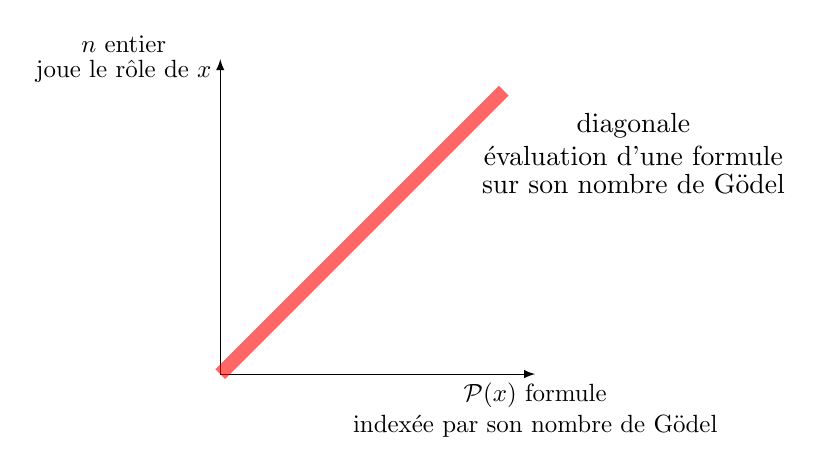
\begin{tikzpicture}[scale=0.8]
    % Axes
    \draw[->,>=latex] (0,0) -- (5,0) node[right] {$\Nn$} node[below,scale=0.9] {\shortstack{$\mathcal{P}(x)$ formule\\indexée par son nombre de Gödel}};
    \draw[->,>=latex] (0,0) -- (0,5) node[above] {$\Nn$} node[left,scale=0.9] {\shortstack{$n$ entier\\joue le rôle de $x$}}
    ;
    % Diagonale
    \draw[line width=5pt, red, opacity=0.6] (0,0) -- (4.5,4.5);
    \node[right] at (4,3.5) {\shortstack{diagonale\\évaluation d'une formule\\sur son nombre de Gödel}};
\end{tikzpicture}
\end{center}


D'où vient cette idée de la diagonalisation ? Elle est déjà présente dans le paradoxe de Russell où la question \og{}Est-ce que $x \in y$ ?\fg{} donne sur la diagonale \og{}Est-ce que $y \in y$ ?\fg{}. Cette méthode a surtout été utilisée par Cantor pour prouver que l'ensemble des réels n'est pas dénombrable. Étudions sa preuve.
\begin{theoreme}
    $\Rr$ n'est pas dénombrable.
\end{theoreme}

\begin{proof}
Supposons par l'absurde que l'ensemble des réels $[0,1[$ soit un ensemble dénombrable, c'est-à-dire en bijection avec $\Nn$.
En termes plus familiers, cela signifie que tous les réels de $[0,1[$ peuvent être numérotés $x_0, x_1, x_2, \dots$
c'est-à-dire $[0,1[ = \{x_k\}_{k \in \Nn}$.

On écrit chaque réel de $[0,1[$ par son écriture décimale, par exemple 
\begin{align*}
x_0 &= 0.189~335\dots \\
x_1 &= 0.772~004\dots \\
x_2 &= 0.191~542\dots \\
x_3 &= 0.053~477\dots
\end{align*} 

Cette écriture décimale est unique si on s'interdit l'écriture avec une infinité de $9$ à la fin.  
Par exemple pour $x=0.123~999~999\dots$ on choisit l'écriture $x=0.124~000~000\dots$ 
On remplit un tableau avec les décimales de tous les $(x_k)_{k \ge 0}$ (sans le $0$ avant la virgule). 


\begin{center}
    \newcommand{\inblue}[1]{\textcolor{blue}{\textbf{#1}}}
    \newcommand{\inred}[1]{\textcolor{red}{\textbf{#1}}}
    \newcommand{\ingray}[1]{\textcolor{gray}{#1}}
\begin{tabular}{c|cccccc}
\vdots & & & & & & \\
\vdots & & & & & & \\
$x_3$ & 0 & 5 & 3 & \inblue{4} & 7 & 7 \\
$x_2$ & 1 & 9 & \inblue{1} & 5 & 4 & 2 \\
$x_1$ & 7 & \inblue{7} & 2 & 0 & 0 & 4 \\
$x_0$ & \inblue{1} & 8 & 9 & 3 & 3 & 5 \\
\hline
& \multicolumn{6}{c}{Décimales} \\
\end{tabular}
\qquad\qquad
\begin{tabular}{c|cccccc}
\vdots & & & & & & \\
\vdots & & & & & & \\
\hphantom{$x_3$} & \ingray{0} & \ingray{5} & \ingray{3} & \inred{1} & \ingray{7} & \ingray{7} \\
 & \ingray{1} & \ingray{9} & \inred{2} & \ingray{5} & \ingray{4} & \ingray{2} \\
 & \ingray{7} & \inred{1} & \ingray{2} & \ingray{0} & \ingray{0} & \ingray{4} \\
 & \inred{2} & \ingray{8} & \ingray{9} & \ingray{3} & \ingray{3} & \ingray{5} \\
\hline
& \multicolumn{6}{c}{\vphantom{Décimales}} \\
\end{tabular}
\end{center} 

Ensuite, on change le chiffre numéro $k$ de $x_k$ selon la règle suivante : 
\begin{itemize}
    \item si ce chiffre est $1$, on le change en $2$, 
    \item et si ce chiffre est différent de $1$, on le change en $1$. 
\end{itemize}

Avec ce procédé on peut lire les décimales d'un nouveau réel $x' \in [0,1[$ sur la diagonale. Sur notre dessin ce serait $x' = 0.2121\dots$ 

Mais par construction $x'$ ne peut pas être l'un des $x_k$ car $x'$ et $x_k$ ont leur décimale numéro $k$ distincte.  C'est une contradiction car $\{x_k\}_{k \in \Nn}$ devait énumérer tous les réels de $[0,1[$. Conclusion : $[0,1[$ n'est pas dénombrable et par conséquent $\Rr$ non plus. 
\end{proof}

%%%%%%%%%%%%%%%%%%%%%%%%%%%%%%%%%%%%%%%%%%%%%%%%%%%%%%%%%%%%%%%%%%%%%
%\section*{Exercices}


\end{document}